\documentclass[12pt, a4paper]{article}
\usepackage{../../../myconfig} % Gọi file cấu hình từ ngoài gốc vào

% ==========================================
% BẮT ĐẦU NỘI DUNG TÀI LIỆU
% ==========================================
\begin{document}

% Truyền 3 tham số: {Nhãn cam} {Chữ to chính giữa} {Chữ ở góc phải Header}
\titlebox{Chủ đề: Hàm số}{Tốc độ nước dâng}{Hàm số: Tốc độ nước dâng}

\drawdashlines{25}
\newpage
\drawdashlines{30}
\newpage
% --- CÂU 1 ---
\questionShortAnswer{20}{1}{Một cái máng dạng hình lăng trụ, trong đó hai đầu của máng là tam giác cân, với đáy 3 m và chiều cao 4 m, và chiều dài của máng là 10 m. Nước đang được bơm vào máng với tốc độ \( 5 \, \text{m}^3 / \text{phút} \). Hỏi tốc độ thay đổi chiều cao của mực nước là bao nhiêu m/phút khi mực nước đang ở độ cao 1 m? (Kết quả làm tròn đến hàng phần trăm).
\begin{figure}[htbp]
    
    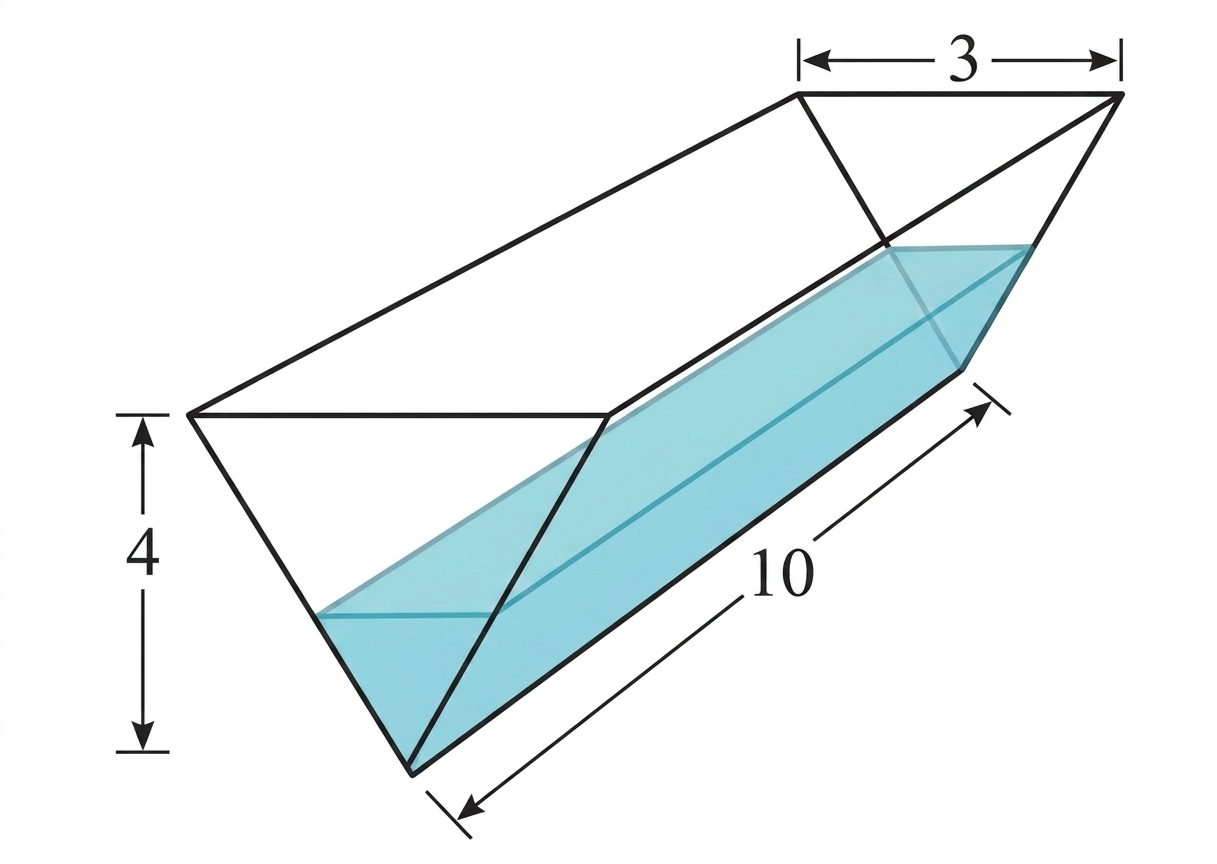
\includegraphics[width=0.4\textwidth]{../images/Cau1nuocdang.png}
    
\end{figure}

}
\newpage
\drawdashlines{30}
\newpage

% --- CÂU 2 ---
\questionShortAnswer{20}{2}{Anh Huy có một bể nước hình nón ngược với bán kính đáy bằng 2 m và chiều cao bằng 4 m. Ban đầu bể không có nước. Anh Huy tiến hành bơm nước vào bể với tốc độ không đổi \( 2 \, \text{m}^3 / \text{phút} \).

a) Hỏi tại thời điểm 4 phút, mực nước trong bể cao bao nhiêu? (đơn vị m)

b) Hỏi tại thời điểm 5 phút, tốc độ dâng lên của mực nước trong bể bằng bao nhiêu? (đơn vị m / phút)
\begin{figure}[htbp]
    
    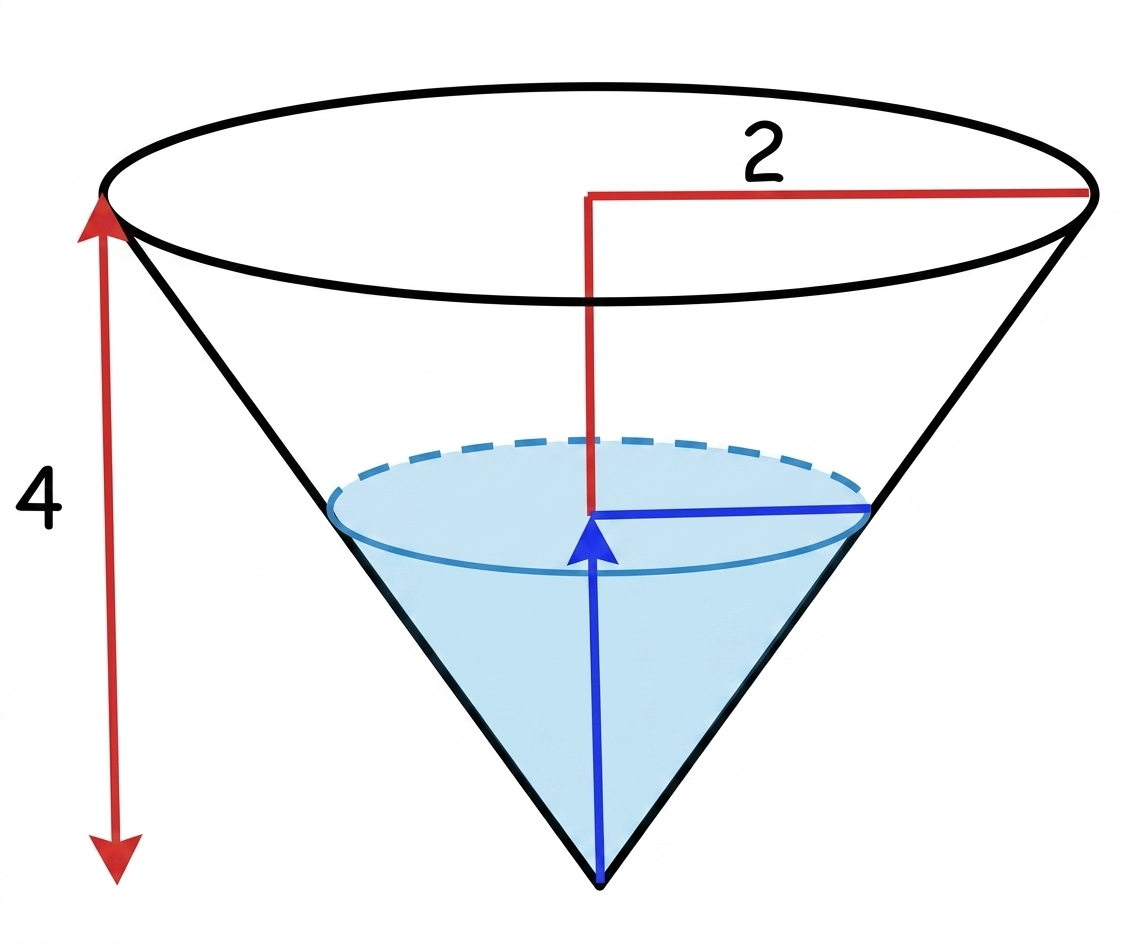
\includegraphics[width=0.4\textwidth]{../images/Cau2nuocdang.png}
    
\end{figure}}
\newpage
\drawdashlines{30}
\newpage

% --- CÂU 3 ---
\questionShortAnswer{20}{3}{Có một cái bể hình chóp cụt đều với đáy dưới (đáy nhỏ) là hình vuông cạnh bằng 30 cm, đáy trên (đáy lớn) có cạnh bằng 60 cm và chiều cao bằng 100 cm. Ban đầu bể không có nước. Người ta tiến hành bơm nước vào bể với tốc độ không đổi \( 2000 \, \text{cm}^3 / \text{phút} \).

a) Hỏi tại thời điểm 10 phút, mực nước trong bể cao bao nhiêu? (đơn vị cm)

b) Hỏi tại thời điểm 7 phút, tốc độ dâng lên của mực nước trong bể bằng bao nhiêu? (đơn vị cm/phút).
\begin{figure}[htbp]
    
    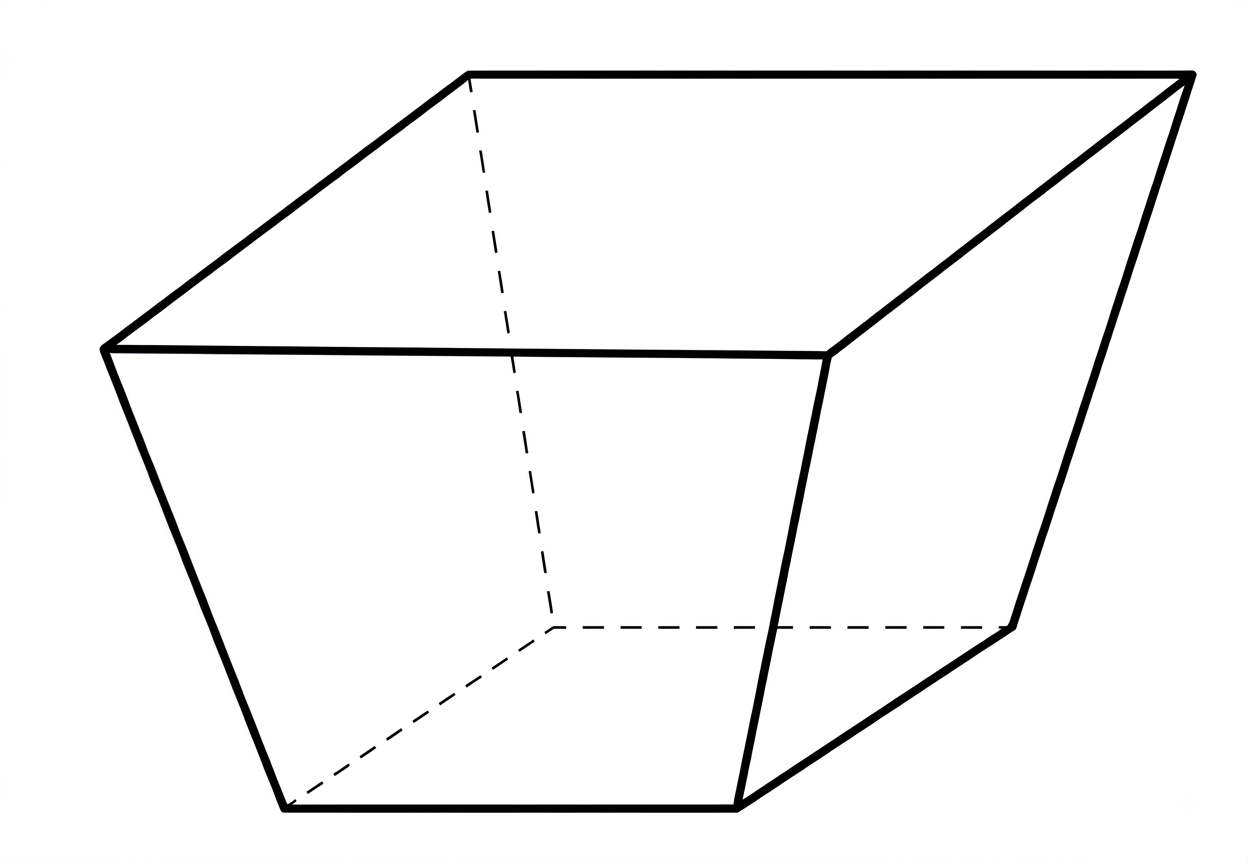
\includegraphics[width=0.4\textwidth]{../images/Cau3nuocdang.png}
    
\end{figure}}
\newpage
\drawdashlines{30}
\newpage

% --- CÂU 4 ---
\questionShortAnswer{20}{4}{Mặt bể bơi của một dự án chung cư cao cấp có dạng một hình chữ nhật với chiều dài 25 m và chiều rộng 8 m. Bể bơi sâu 1 m ở bên đầu nông và sâu 2 m bên đầu sâu, đáy dốc đều theo chiều dài của bể bơi (hình vẽ). Ban đầu bể không có nước, nước bắt đầu được bơm vào bể vào lúc 7 giờ sáng với tốc độ 1 m³ mỗi phút. Vào lúc 8 giờ 4 phút sáng thì mực nước dâng lên với tốc độ \(\dfrac{1}{a}\) m/phút. Giá trị của \(a\) bằng bao nhiêu?
\begin{figure}[htbp]
    
    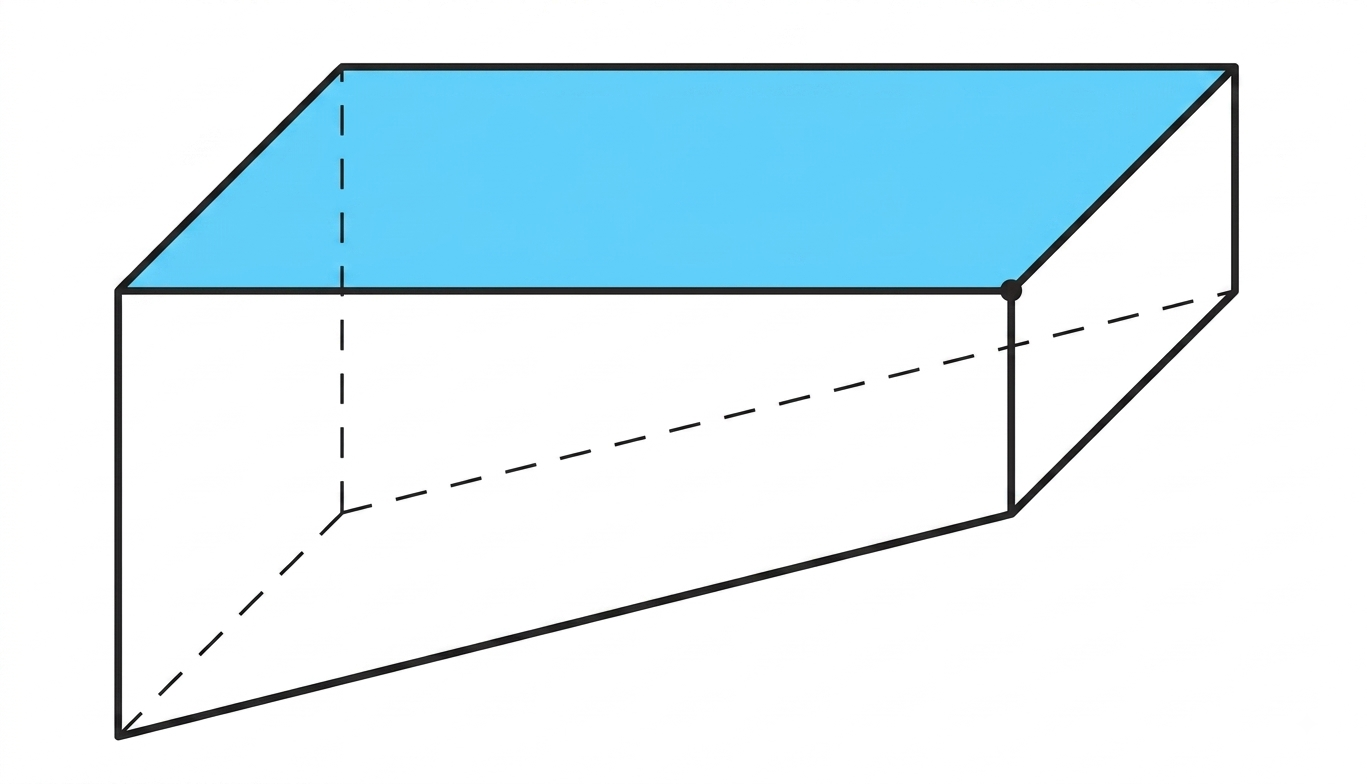
\includegraphics[width=0.4\textwidth]{../images/Cau4nuocdang.png}
    
\end{figure}}
\newpage
\drawdashlines{30}
\newpage


\end{document}